\chapter{Analyse}
\label{ch:analyse}

In dit hoofdstuk wordt alles omtrent de analyse uitgelegd en beschreven. 

Voor we begonnen aan de effectieve implementatie werd een backlog gemaakt en hebben we gebruik gemaakt van wekelijkse sprints, die starten op woensdag en eindigden precies zeven dagen later. Sander Brugge nam de rol op zich van scrummaster, hij besliste welke tickets die week werden opgenomen en dan kon onderling beslist worden wie wat deed. Ook besliste hij welke tickets de hoogste prioriteit hadden en wat zeker af moest zijn.

Elke week maakte hij een nieuwe sprint aan in Trello, en zorgde ervoor dat via burndown for Trello de vooruitgang kon bekeken worden en dat er een burndown gegenereerd werd. Elke woensdag op het einde van een sprint hielden we ook een retrospective, om te kijken wat goed ging, wat minder goed ging en wat we gaan doen. Deze zijn allemaal terug te vinden in volgende sectie.

Alle communicatie verliep via de proffesionele team communicatie tool Slack. Aangezien iedereen binne het team relatief ver van elkaar wonen. Voor quality assurance werd gebruik gemaakt van Pull Requests op Github. Waar iedereen commentaar kon schrijven, verbeteringen kon voorstellen of meer uitleg vragen over bepaalde stukken code.

\section{Sprints}

in onderstaande sectie zijn de backlog, burndown en retrospective terug te vinden per sprint. De taken werden onderling verdeeld en besproken via Slack.

\paragraph{Sprint 1}
De eerste week hebben we fysiek samengezeten om de startup te bespreken en te discussiëren wat we van de app verwachten. Na de tijd te hebben genomen om de opdracht te bekijken en te beluisteren, kwamen we tot een algemeen idee. Zoals beschreven in het hoofdstuk plan van aanpak. Op basis van ons idee hebben we een backlog gemaakt met de belangrijkste use cases. Voor ons was het sociale aspect zeer belangrijk. Zo kan een gebruiker inloggen via Facebook en Vegagram posts delen op Facebook om andere mensen aan te zetten tot het gebruik van de app of een veganistische levensstijl.


De backlog van de eerste sprint. Hier is direct zichtbaar dat alles in de backlog gestoken wordt, zowel functionele requirements maar ook niet functionele. Een voorbeeld hiervan is het bespreken van de app. Ook hier moet tijd voor gerekend worden in de sprint.

\begin{figure}[H]
\centering
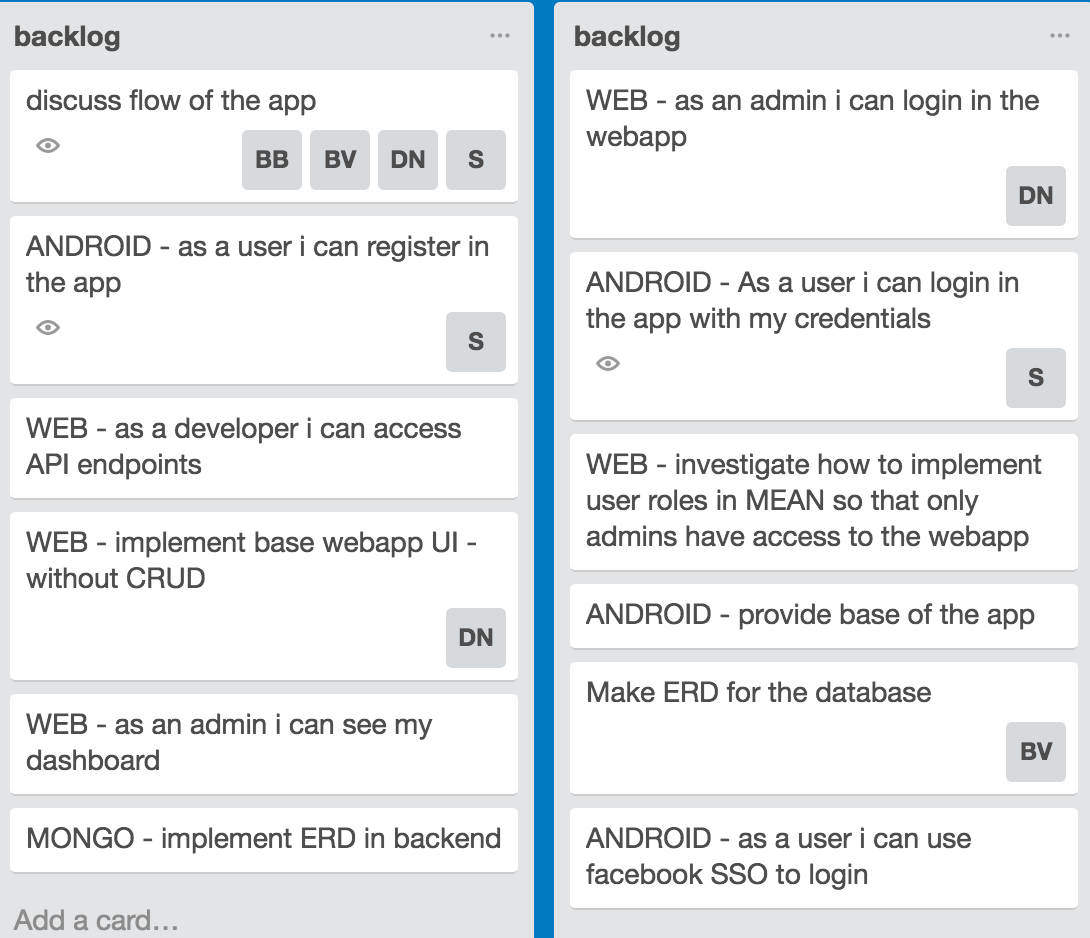
\includegraphics[width=15cm]{img/backlog_week1.png}
\caption{backlog sprint 1}
\end{figure}

De burndown is niet perfect omdat dit de eerste week was en er iets te veel hooi op de vork werd genomen. 

\begin{figure}[H]
	\centering
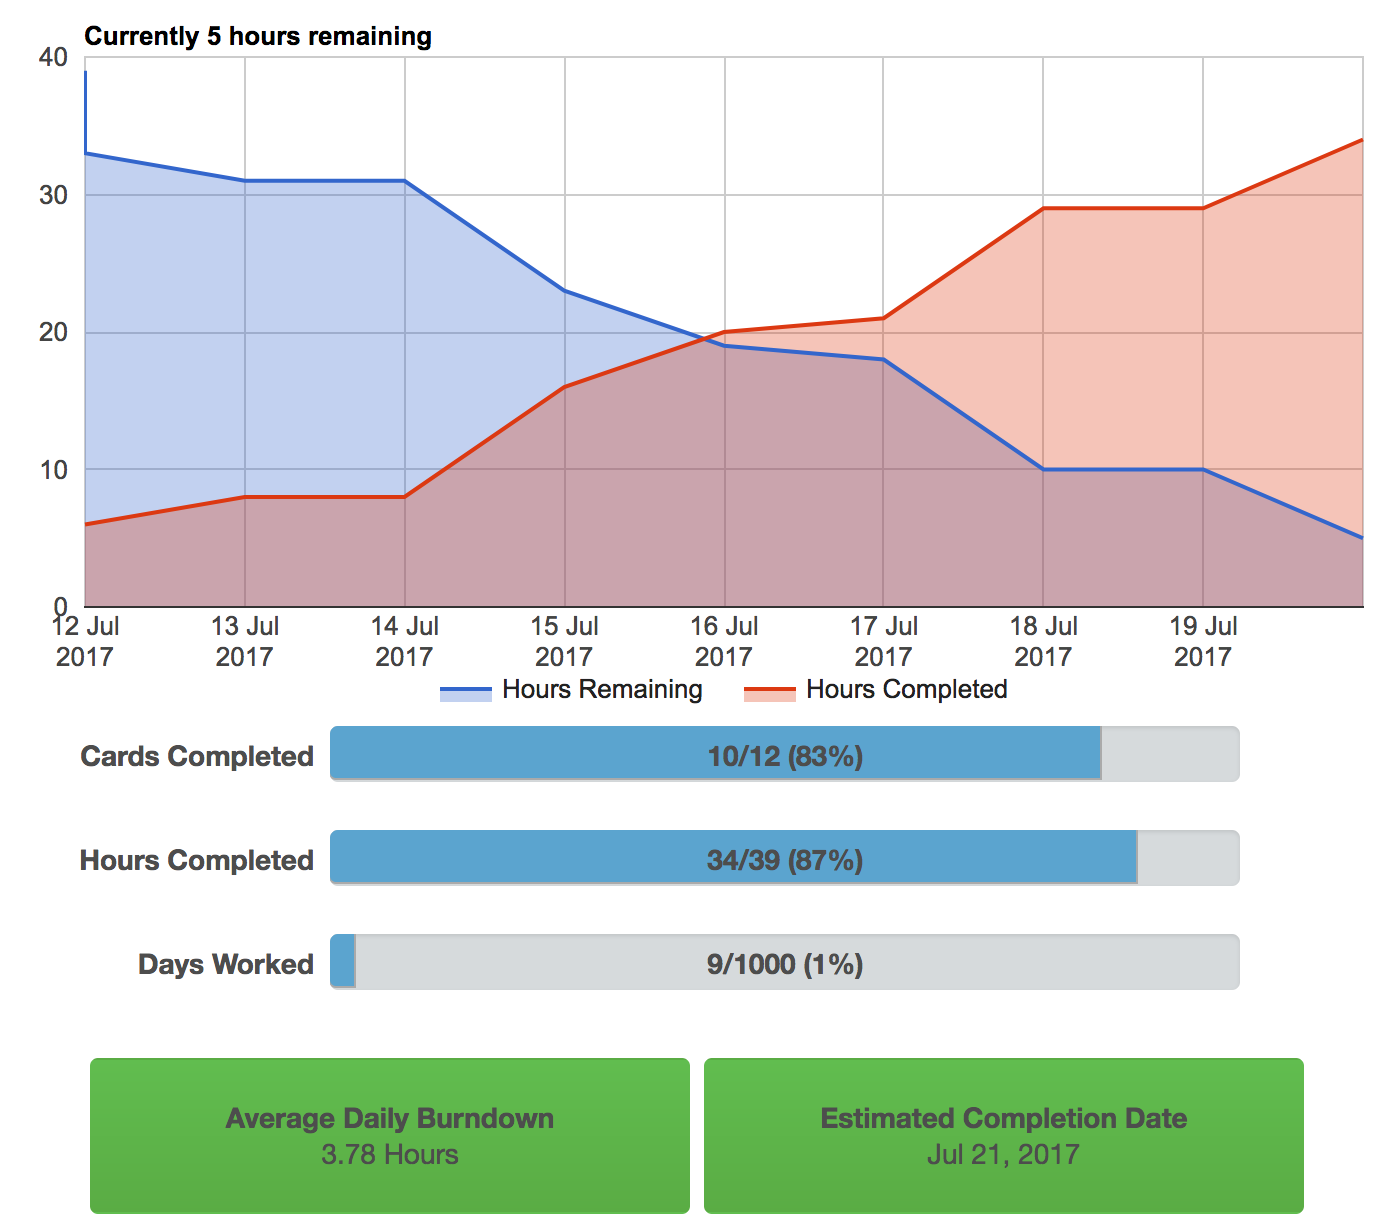
\includegraphics[width=15cm]{img/burndown_week1.png}
\caption{burndown sprint 1}
\end{figure}

Op het einde van een sprint vond ook altijd een retrospective klaar, daarvan is een kort verslag te vinden hieronder.

Sprint 1:
What did we do good

\begin{itemize}
\item Begonnen met goed idee
\item Fysiek samen zitten om het plan te bespreken
\item Vertrokken van uit de basis (ERD/goede afspraken)
\item  Agile werken
\item Best practices respecteren van in het begin
\end{itemize}

What could we have done better

\begin{itemize}
\item Beter inplannen van de tickets
\item Beter verdelen van taken
\item Rekenen op meer tijd voor mooiere UI
\end{itemize}

\paragraph{Sprint 2}
De backlog van de tweede sprint. Dit ziet er op eerste zicht een veel kleinere backlog uit maar de tickets die beschreven zijn waren veel zwaarder en groter van omvang. Hier werd de basis van alles geïmplementeerd dus dit moest ook correct zijn van in het begin.

\begin{figure}[H]
	\centering
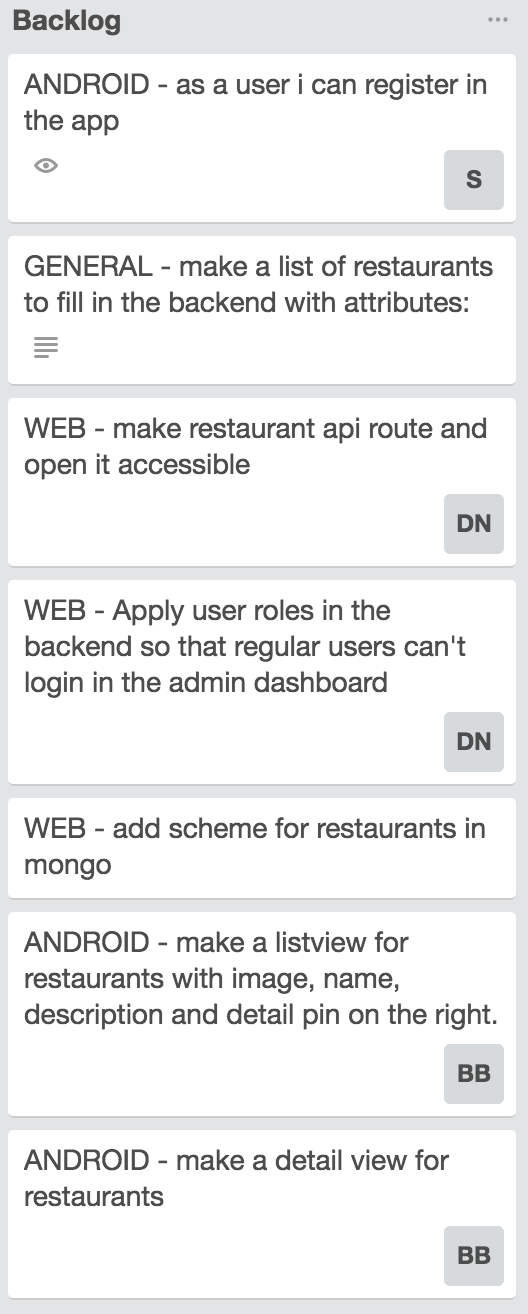
\includegraphics[width=7cm,height=18cm]{img/backlog_week2.png}
\caption{backlog sprint 2}
\end{figure}

Dit ziet er ook al beter ingeschat uit dan de eerste sprint, we maken snel voorruitgang als team!

\begin{figure}[H]
	\centering
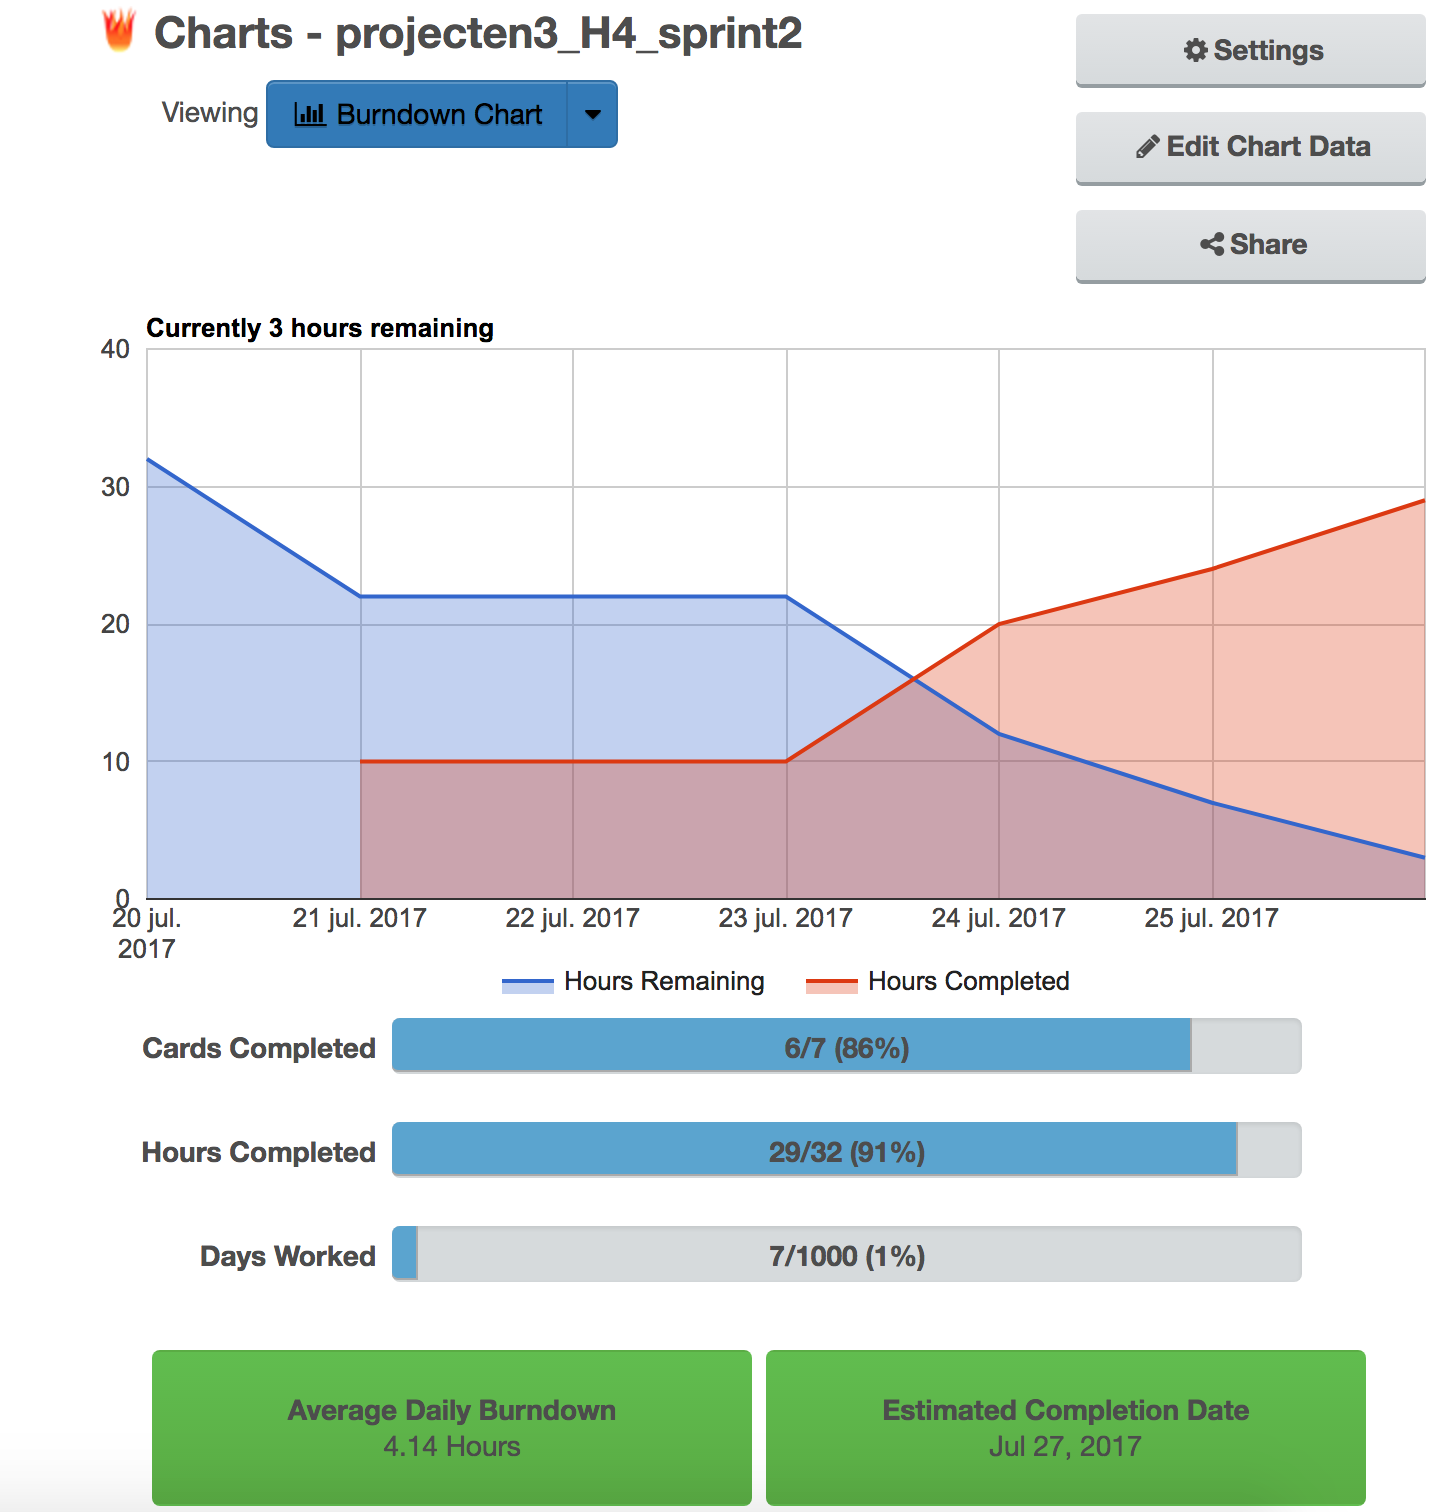
\includegraphics[width=15cm]{img/burndown_week2.png}
\caption{burndown sprint 2}
\end{figure}

Ook hier was na het einde van deze sprint een retrospective, die gehouden werd via Slack.

Sprint 2:

What did we do good
\begin{itemize}
\item met branches werken
\item pull requests om elkaar code te reviewen
\item goed de sprint gepland
\item  goede communicatie dmv Slack
\end{itemize}

what could we have done better

\begin{itemize}
\item betere UI van in begin
\item sommige zaken (zoals properties in pojo's) bespreken in slack ipv in commentaar in de code
\item Javadoc toevoegen test
\end{itemize}


\paragraph{Sprint 3}
De backlog van de derde sprint.

\begin{figure}[H]
	\centering
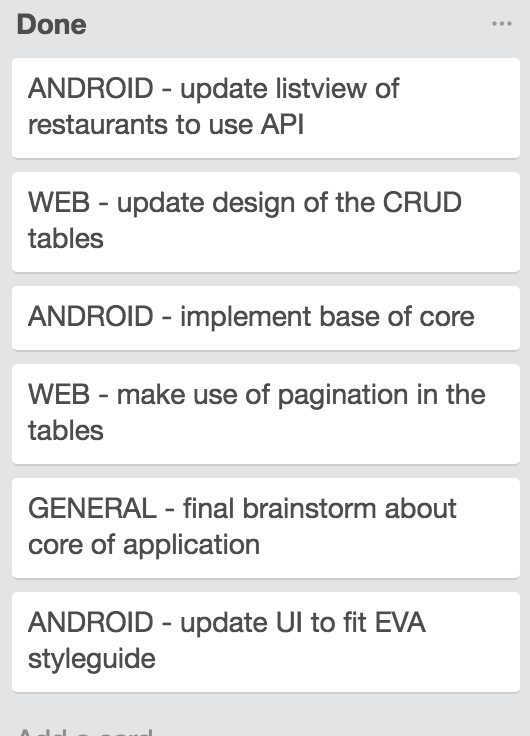
\includegraphics[width=10cm,height=15cm]{img/backlog_week3.png}
\caption{backlog sprint 3}
\end{figure}

Zoals te zien aan de burndown van deze sprint hadden we te weinig opgenomen voor deze sprint. De scrummaster heeft dan beslist dat er extra tickets bij genomen mochten worden. Dit zorgt voor een piek in de grafiek.

\begin{figure}[H]
	\centering
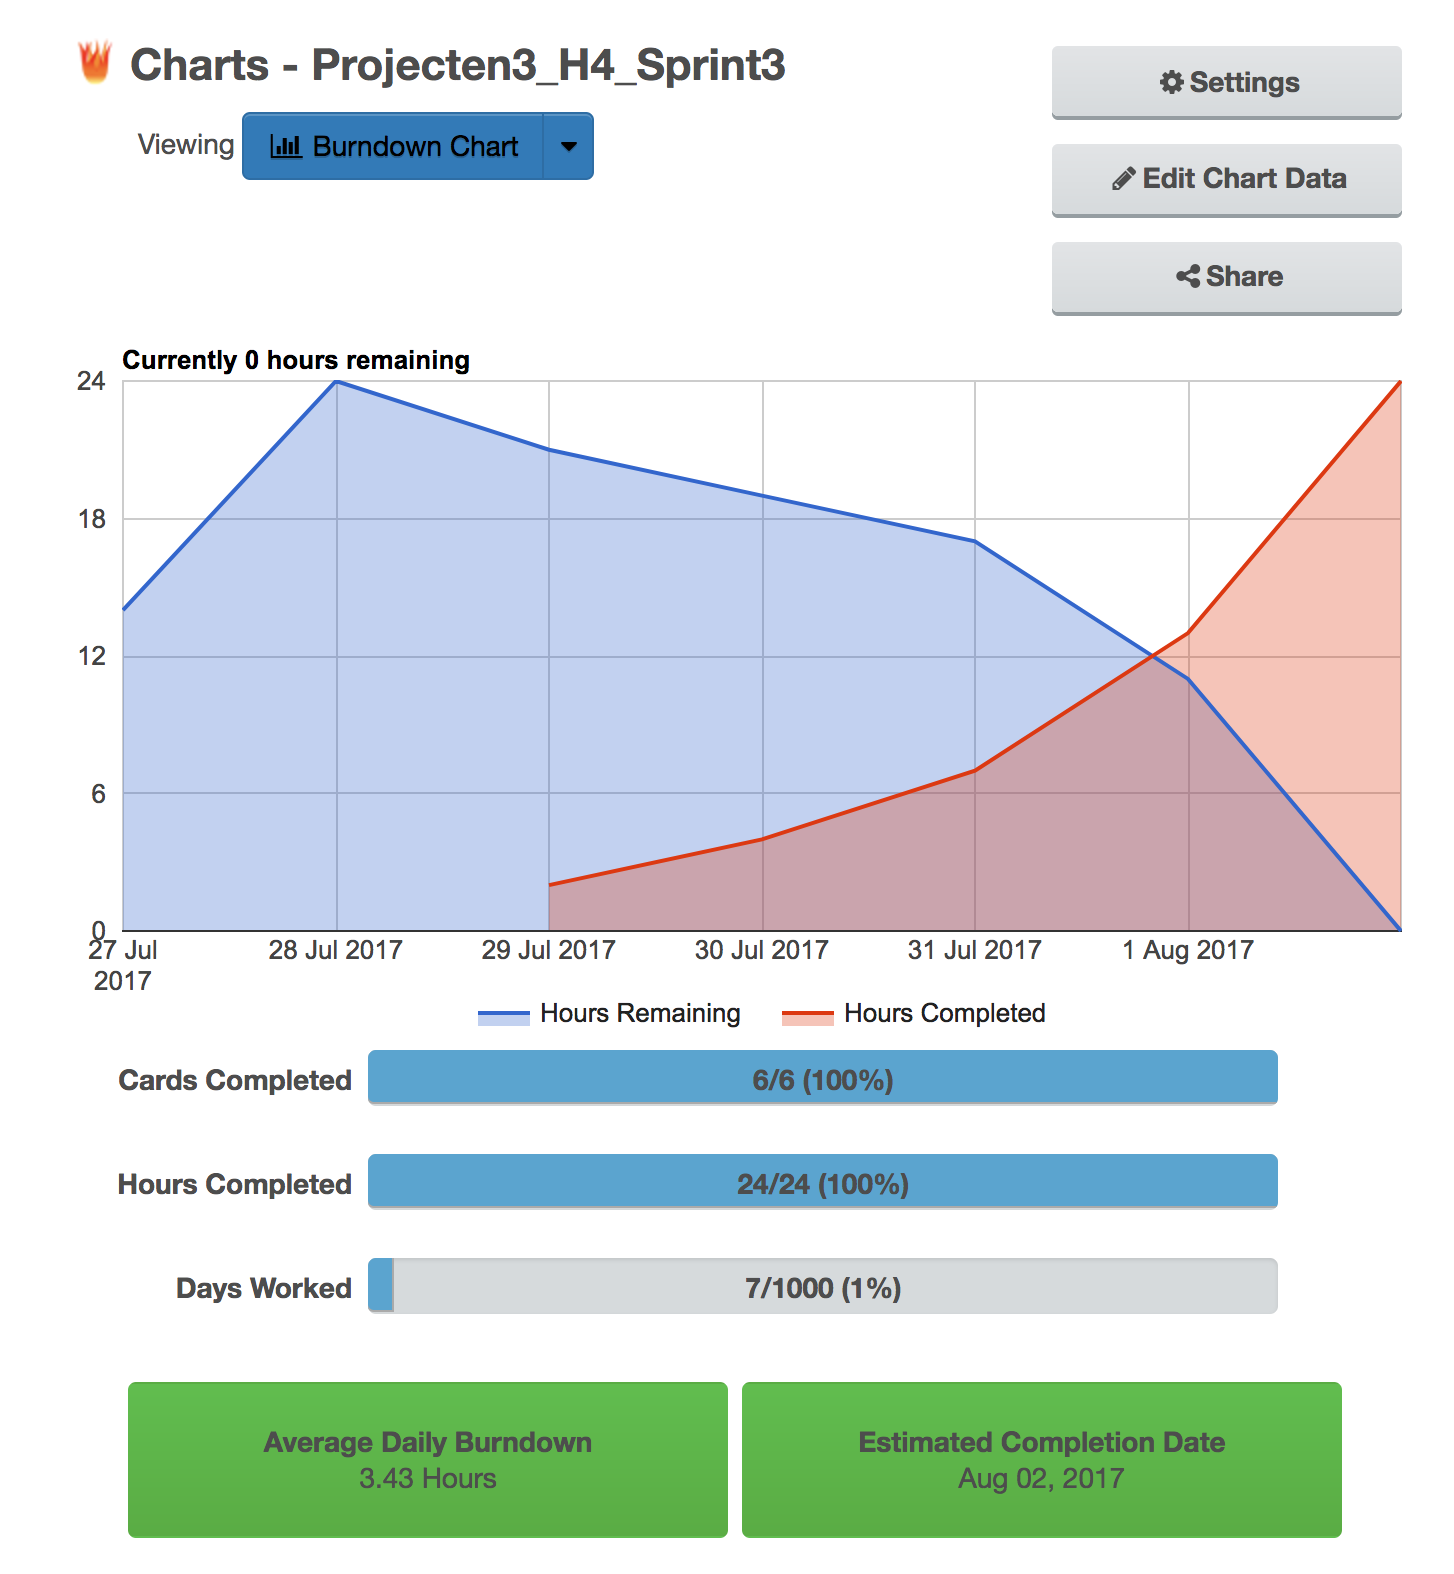
\includegraphics[width=15cm]{img/burndown_week3.png}
\caption{burndown sprint 3}
\end{figure}

Op het einde van de sprint werd opnieuw een retrospective gehouden. Dit zal aanhouden gedurende de volgende sprints ook.

sprint 3:

What did we do good

\begin{itemize}
\item  beter rekening gehouden met de UI en javadoc
\item  coderefactoring van bij de start zodat dat later geen onduidelijke code wordt/blijft
\item verder werken via git flow
\end{itemize}

What could we have done better

\begin{itemize}
\item UI testing
\item unit testing
\item goed webgedeelte en android app laten afstemmen qua properties test
\end{itemize}


\paragraph{Sprint 4}
De backlog van de vierde sprint.

Deze sprint was perfect ingepland en is dan ook tot een goed einde geraakt.

\begin{figure}[h]
	\centering
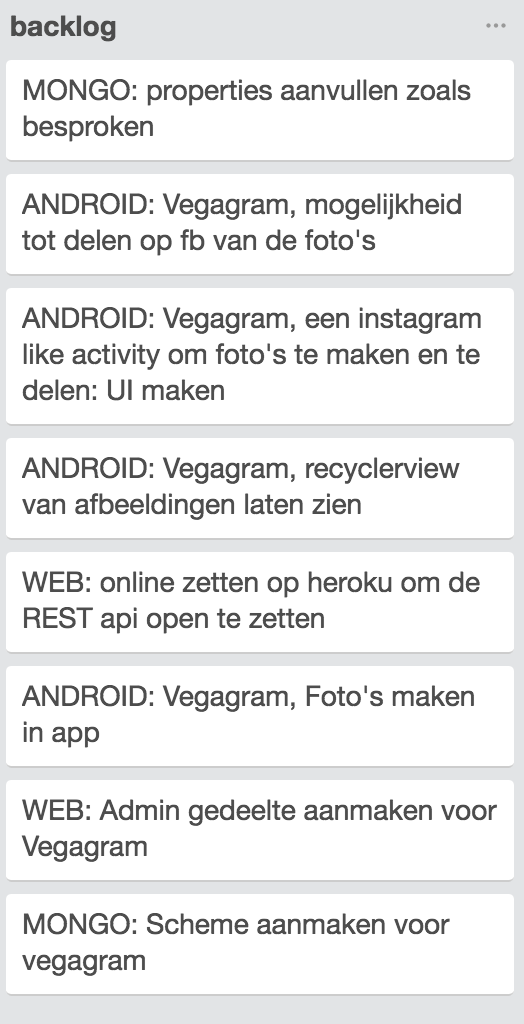
\includegraphics[width=10cm,height=15cm]{img/backlog_week4.png}
\caption{backlog sprint 4}
\end{figure}

Zoals te zien in de burndown ging het werk vlot. Dit is te zien aan de tickets die snel en consistent naar beneden gaan. 

\begin{figure}[h]
	\centering
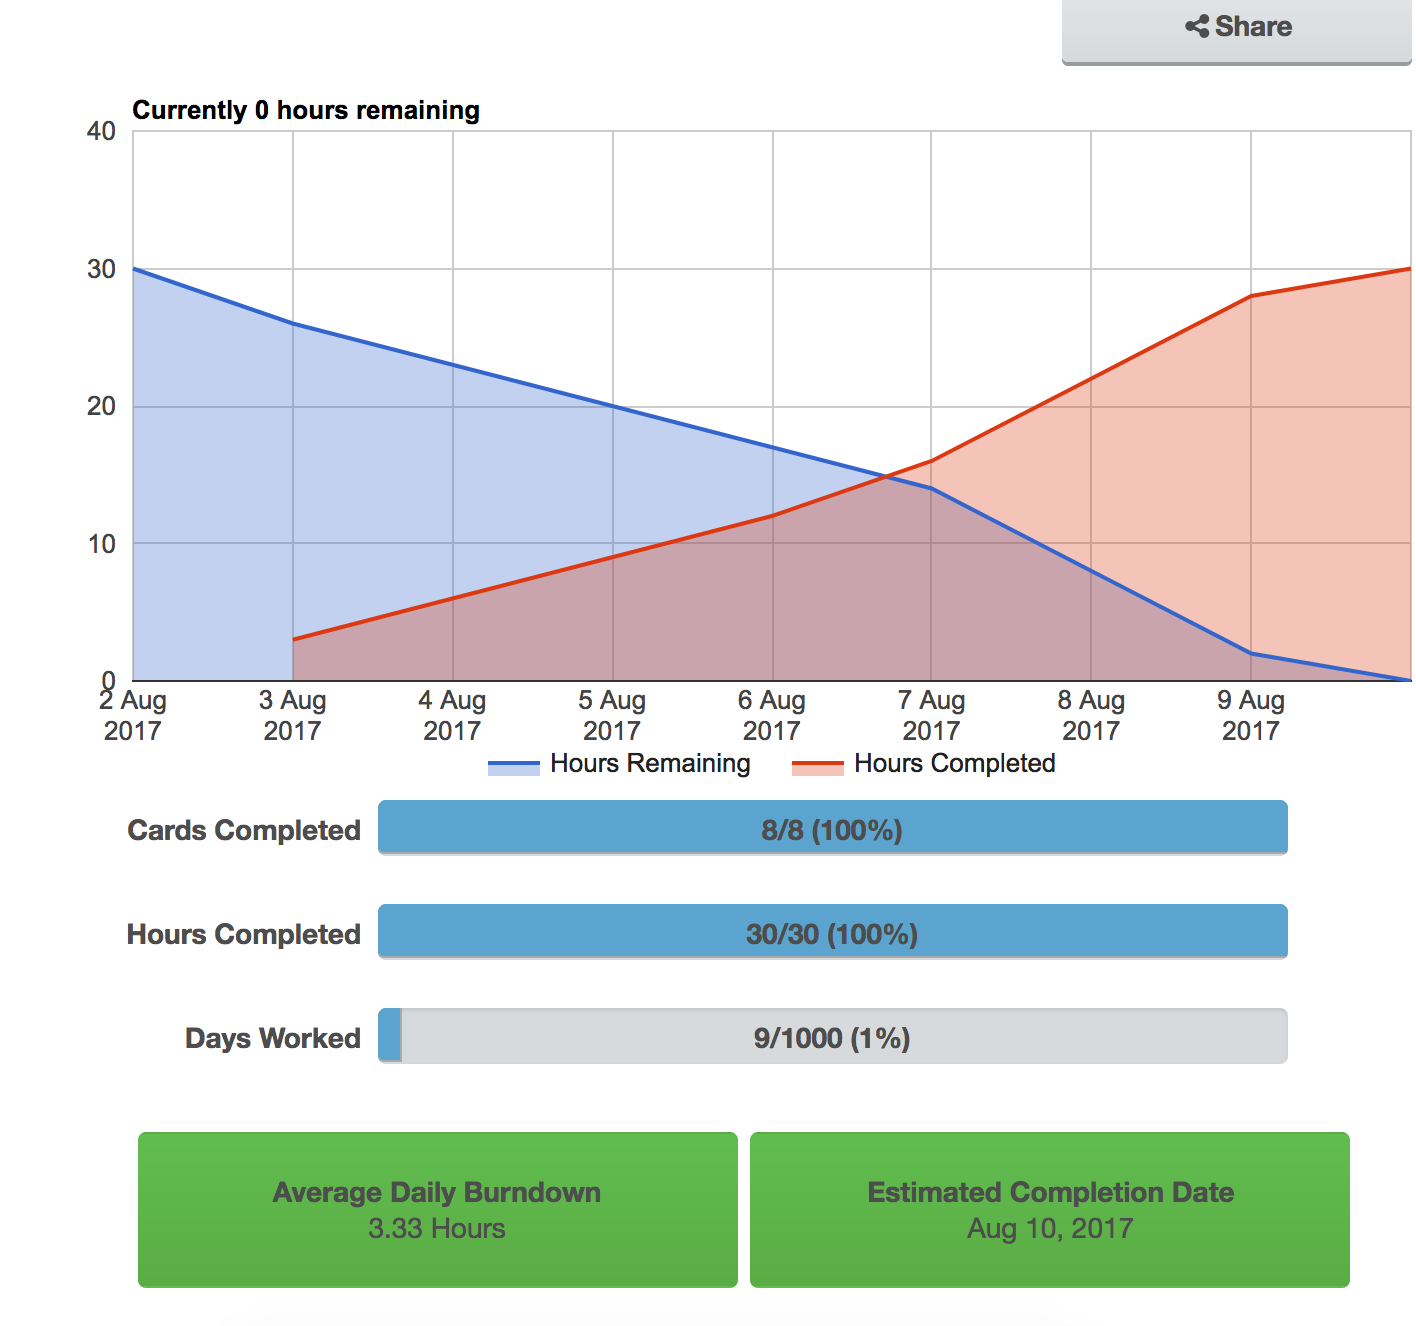
\includegraphics[width=15cm]{img/burndown_week4.png}
\caption{burndown sprint 4}
\end{figure}

Ook hier wordt opnieuw een retrospective besproken.

Sprint 4:

What did we do good:

\begin{itemize}
\item goede communicatie voor backend/frontend
\item coderefactoring van bij de start zodat dat later geen onduidelijke code wordt/blijft
\item pair programming
\item verder werken via git flow
\end{itemize}

What could we have done better

\begin{itemize}
\item UI testing
\item unit testing test
\end{itemize}

\paragraph{Sprint 5}
De backlog van de vijfde sprint.

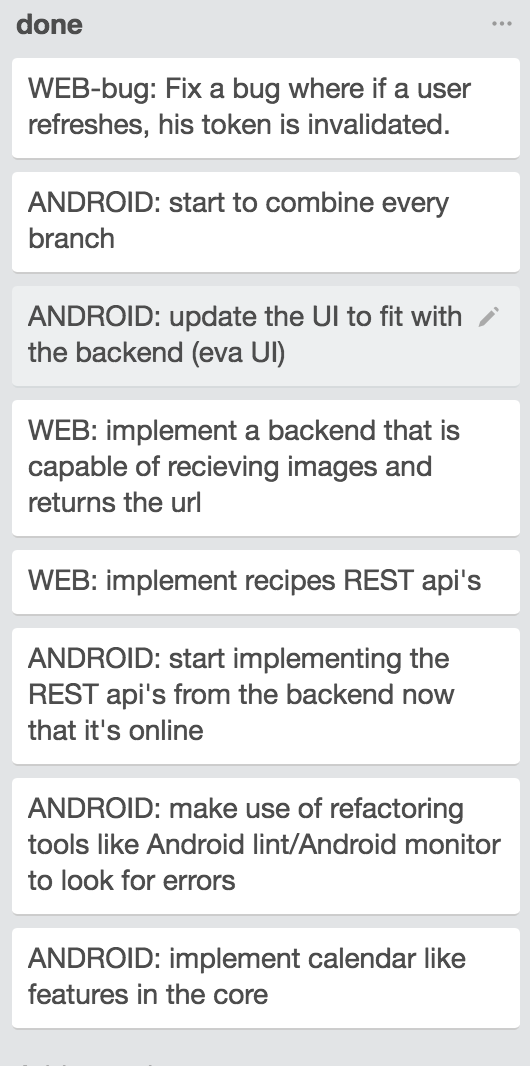
\includegraphics[width=10cm]{img/backlog_week5.png}


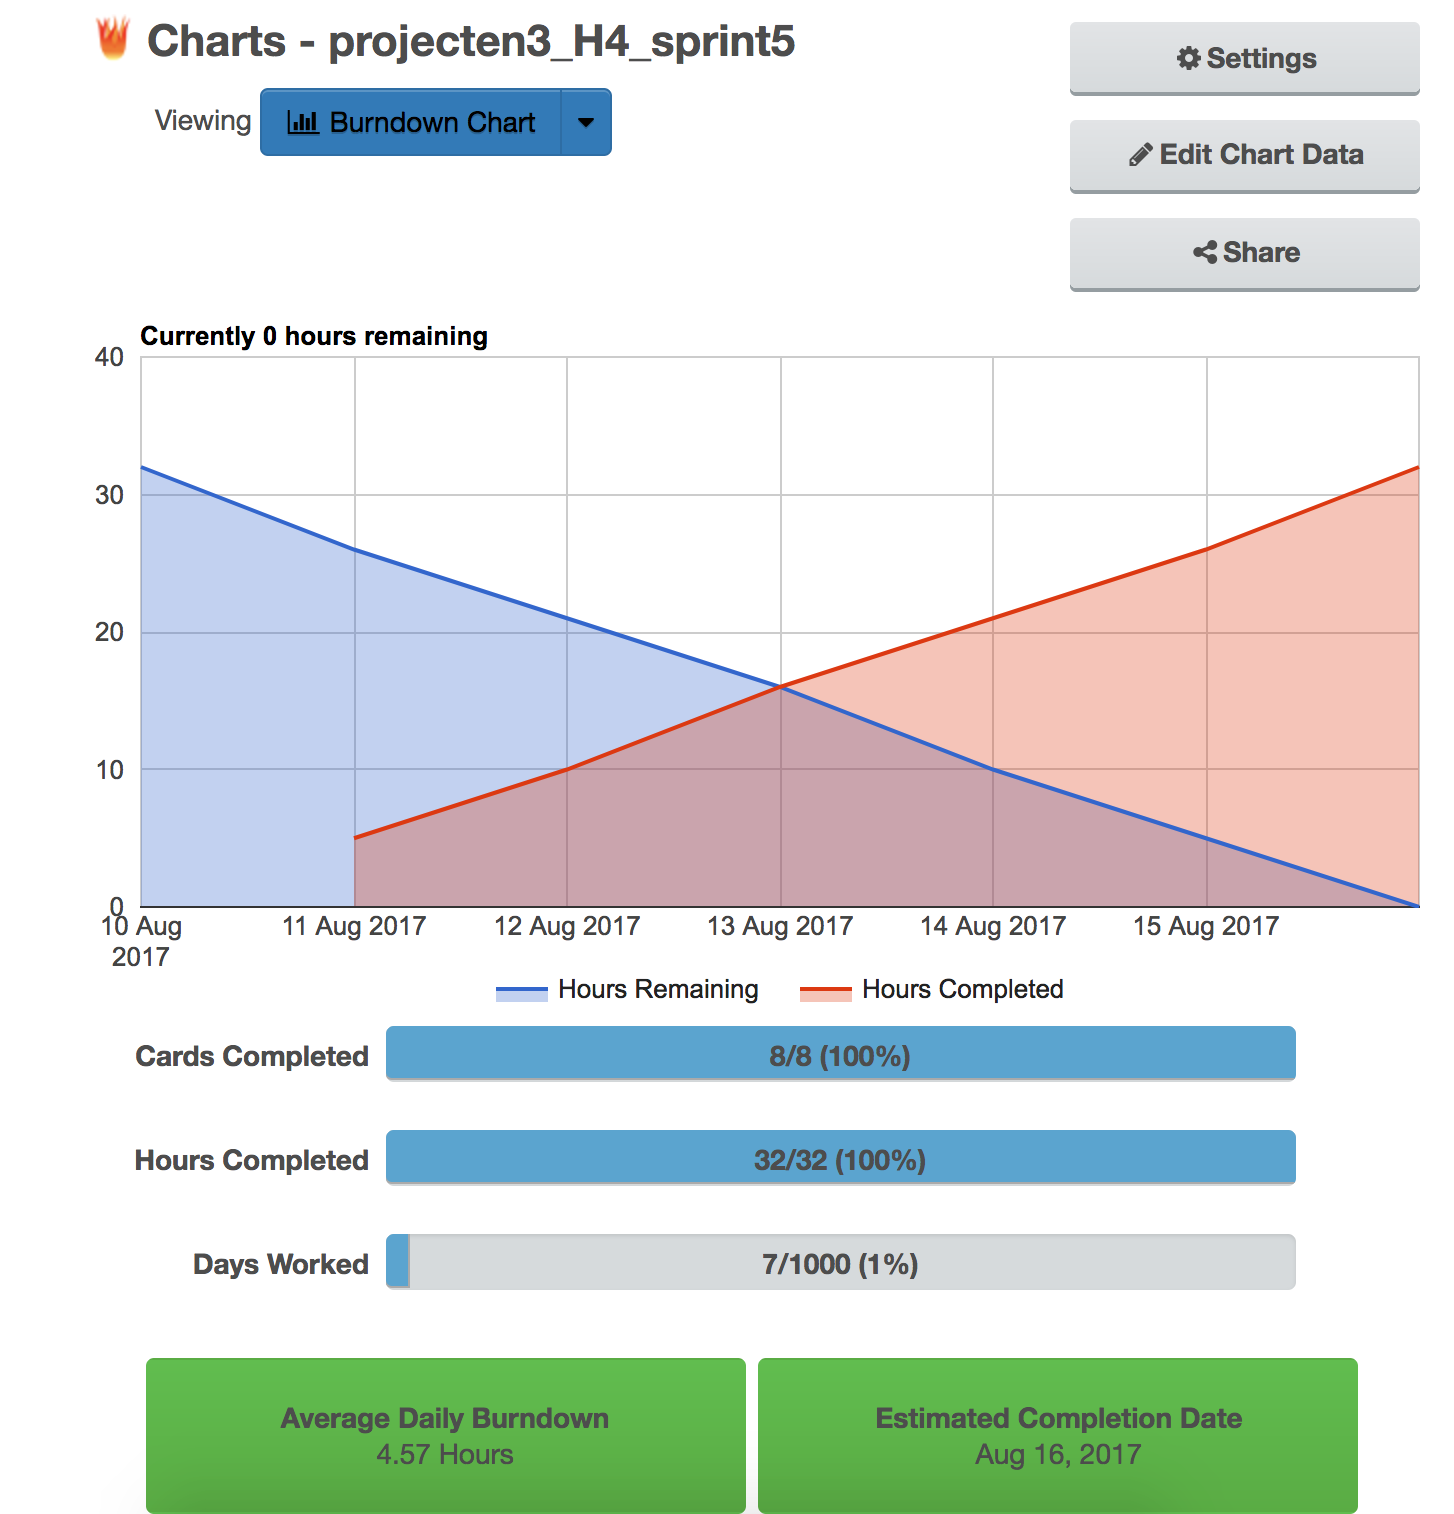
\includegraphics[width=15cm]{img/burndown_week5.png}

sprint 5:

What did we do good:

\begin{itemize}
\item duidelijke taakverdeling
\item mplementatie met best practices in het achterhoofdpair programming
\item verder werken via git flow
\item duidelijke communicatie voor design app in overeenkomst met de backend
\end{itemize}

What could we have done better

\begin{itemize}
\item UI design
\item nog extra javadoc toevoegen
\item beta testing
\end{itemize}
